\chapter{Applikasjon}

Dette kapittelet tar for seg arbeidsgangen i prosjektet, en detaljert arkitekturskisse, og en gjennomgang av all funksjonalitet knyttet til geoprosessering, filbehandling, grensesnitt og brukerveiledning. I tillegg skal det bli snakket om kode-dokumentasjon og hosting av tjenestene på github pages og herokuapp. 

\section{Arbeidsgang}

Det første som ble gjort i forbindelse med applikasjonen var å få en forståelse av hva som har blitt gjort tidligere, med tanke på valg av grensesnitt og funksjonalitet. Dette var også med på å få en forståelse av hva som var forventet og hva som ligger i ordene \textit{viktig GIS-funksjonalitet}. Et dokument som inneholdt geoprosseseringsfunksjonalitet og lagbehandlingsfunksjoner ble laget utifra tilgjengelige prosjekter\cite{Johanessen}\cite{Strand}\cite{Eglaaen}\cite{Villanger}\cite{Jakobsen} som lå tilgengelig på nett.

De ulike geoprosesseringsoperasjonene inkluderte blant annet:

\begin{frame}

    \begin{tabular}{p{0.4\textwidth}p{0.5\textwidth}}

        \begin{itemize}
            \item Clip
            \item Buffer
            \item Union
            \item Dissolve
        \end{itemize} &

        \begin{itemize}
            \item Difference
            \item Intersection
            \item Bounding box
            \item Filtering
        \end{itemize}
    \end{tabular}

\end{frame}

Mens typiske lagbehandlingsfunksjoner var:

\begin{frame}

    \begin{tabular}{p{0.4\textwidth}p{0.5\textwidth}}

        \begin{itemize}
            \item Legge til lag
            \item Fjerne lag
            \item Endre navn på lag
            \item Endre farge på navn
        \end{itemize} &

        \begin{itemize}
            \item Vise/skjule lag
            \item Zoome til lag
            \item Laste ned lag
            \item Fjerne lag
        \end{itemize}
    \end{tabular}

\end{frame}

Etter å ha sjekket at de programmeringsspråkene jeg ønsket å jobbe med hadde støtte for denne typen operasjoner var neste steg å sette opp klient-prosjektet og server-prosjektet. Versjonskontrollsystemet git gir stor fleksibilitet til å prøve og feile, samt holde tidligere versjoner av programmet enkelt tilgjengelig hvis det skulle bli nødvendig å gå tilbake. Begge prosjektene ble knyttet til github, og kildekoden finnes på følgende nettadresser:

\href{https://github.com/torsol/PiG-frontend}{Klient-prosjektet}

\href{https://github.com/torsol/PiG-backend}{Server-prosjektet}

Den neste oppgaven var å få en minimal versjon av klient-programmet til å fungere. Det ble laget et initielt React-program som lastet inn en mapbox-komponent. Se figur \ref{fig:firstmap}. Dette var slik applikasjonen så ut etter den commiten til github 3. september.

\begin{figure}[h]
    \center
    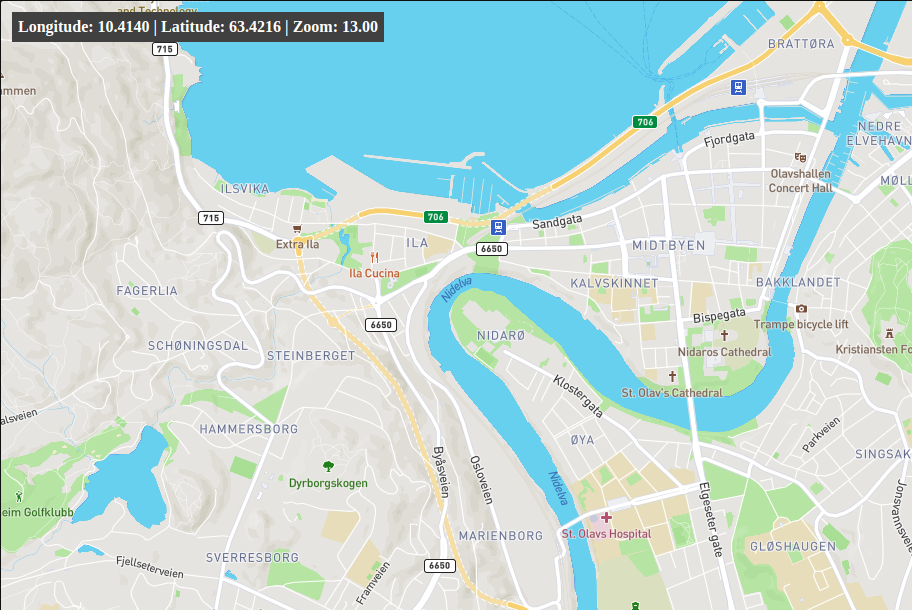
\includegraphics[scale=0.3]{first_frontend.png}
    \caption{Første versjon av klienten}
    \label{fig:firstmap}
\end{figure}

Den neste oppgaven var å få opp Server-prosjektet. Det ble gjort et bevvist valg om å holde programkodene adskilt siden de to applikasjonene i teorien kunne utvikles parallelt. Den aller første kommunikasjonen var et enkelt get-kall til flask-serveren. Som et proof of concept ville et get-kall til '/api/ping' returnere 'pong', see figure \ref{fig:firstping}. Kallet ble gjort via applikasjonen Postman, som er et utviklingsvertkøy for å foreta seg http-kall, dette ble flittig brukt for å teste ulike http-post-kall til serveren gjennom utviklingsprosessen.

\begin{figure}[h]
    \center
    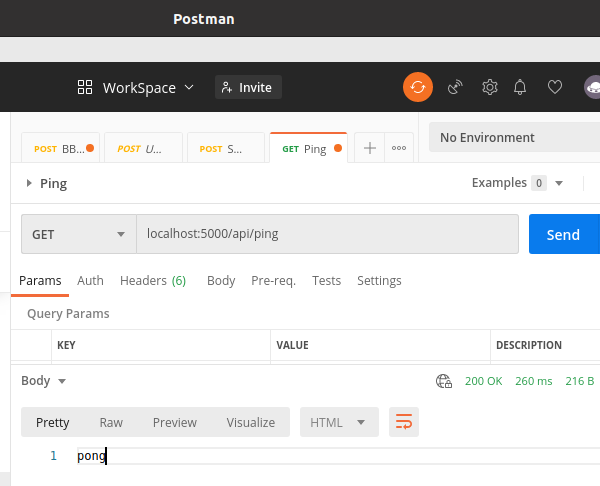
\includegraphics[scale=0.5]{ping.png}
    \caption{Første ping-pong-svar fra server, gjort via Postman}
    \label{fig:firstping}
\end{figure}

Etter at begge prosjektene var oppe og de ulike rammeverkene fungerte isolert, var hovedfokuset på å knytte sammen klient og server, ved å implementere at klienten kunne gjøre egne HTTP-kall for å få data fra serveren. Når også dette fungerte ble det satt opp en løype for å hoste de to tjenestene på github-pages og heroku, slik at man enkelt kunne gjøre nye oppdateringer i applikasjonene tilgjengelig over nett. Mer om dette kommer i seksjon \ref{sec:hosting}.

Når hovedarkitekturen var på plass flyttet fokuset seg over til å implementere mer funksjonalitet og brukergrensesnitt. Funksjonalitet var drevet av de kartlagte funksjonene funnet tidligere i arbeidsprosessen, mens brukergrensesnittet ble laget inspirert av målene om at applikasjonen skulle være brukervennlig og at det skulle bestå av mest mulig interaksjon i kartet.

Videre ble det forberedt data og laget en brukerveiledning som kan finnes både inne i klienten, men også i denne rapporten i appendiks \ref{sec:brukerveiledning}. Helt tilslutt gjenstod det å oppsummere arbeidet i denne rapporten og lansere den endelige versjonen som kan sees i figur \ref{fig:final-version}.

\begin{figure}[h]
    \center
    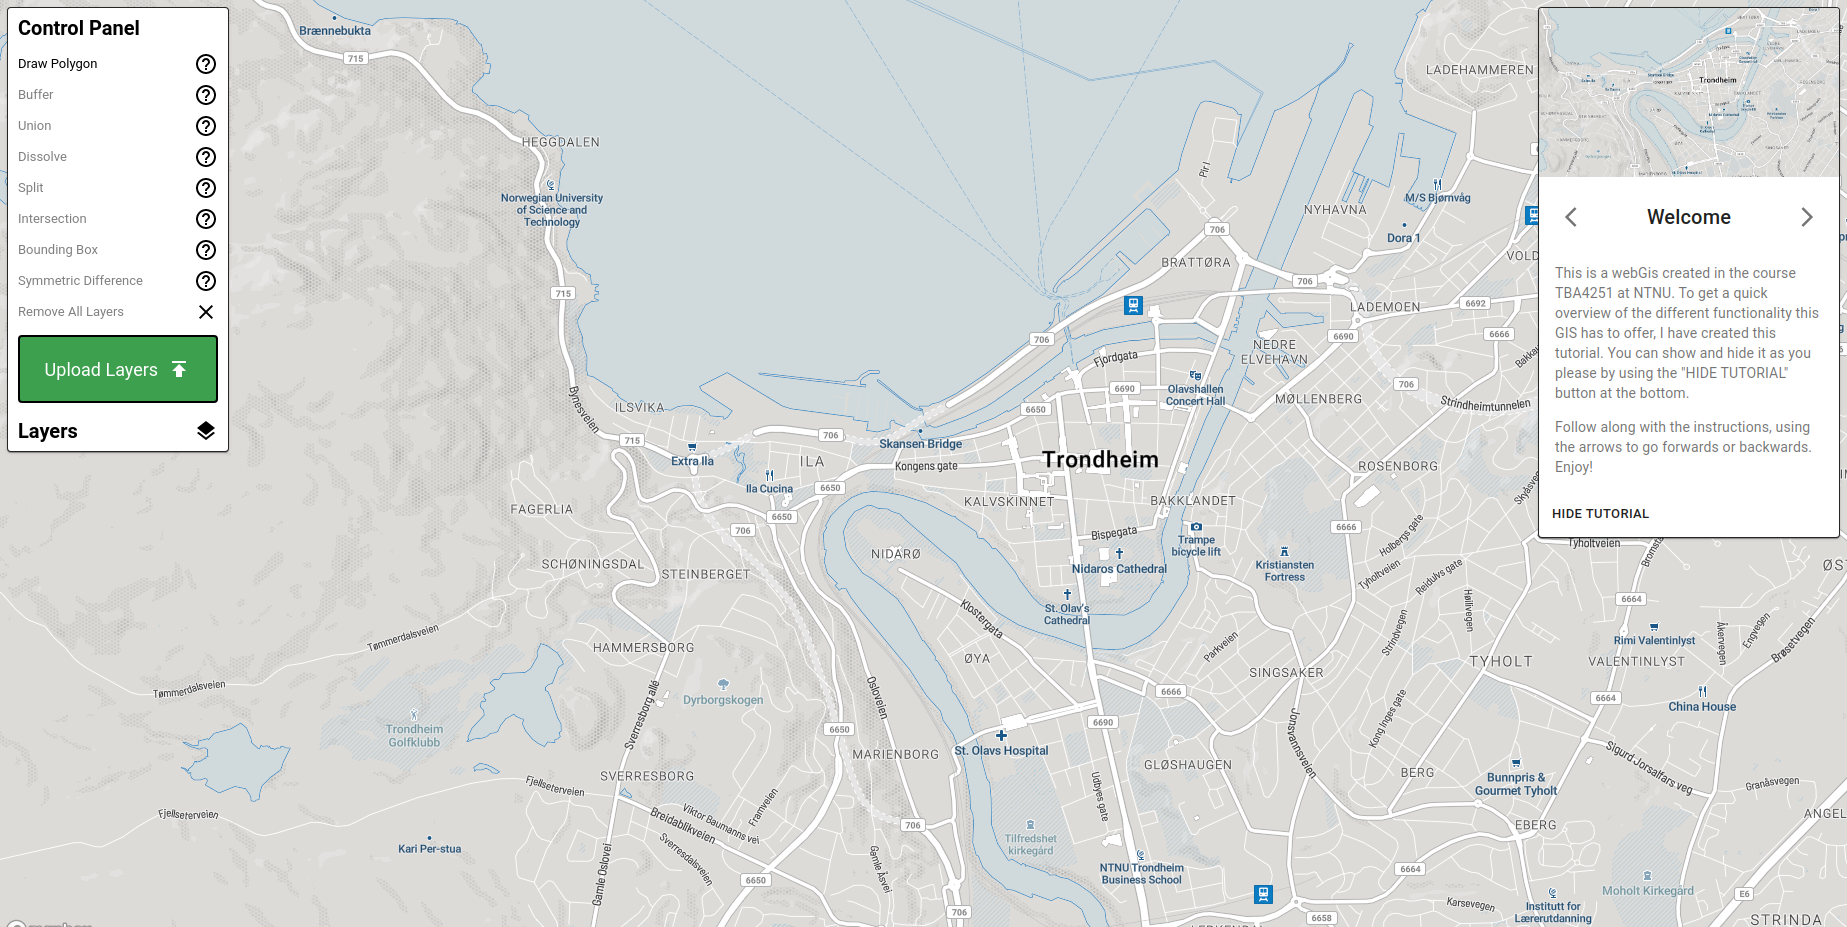
\includegraphics[scale=0.23]{final_version.png}
    \caption{Endelig versjon av prosjektet}
    \label{fig:final-version}
\end{figure}

\section{Detaljert arkitektur}

Klienten er bygget på React, og følger konvensjonene for bruk av komponenter og State-behandling. En komponent i React kan enten være en klasse, eller en funksjon, skrevet i javascript. Deres oppgave er å returnere HTML som vises i nettleseren når man besøker nettsiden. Det som avgjør hvilken HTML som returneres er komponentenes interne State (eller tilstand). Komponenter kan sende informasjon til hverandre og returnere andre komponenter, og det er en konvensjon at informasjon kun skal flyte fra foreldre-komponenten til barn-komponenten og ikke motsatt. En total nettside består gjerne av flere komponenter, der hver komponent har et ansvarsområde.

i figur \ref{fig:react-arkitektur} kan man se den totale komponent-strukturen til klienten. Rot-komponenten App består av komponentene Sidebar, Map og Tutorial. I tillegg har App ansvaret for State til alle kartlagene som legges til. Sidebar-komponenten har hovedansvaret for å vise sidebaren, og består av komponentene Dropzone, Operation og Layerbar. Dropzone er komponenten som behandler filopplastinger. Layerbar er den delen av sidebaren som viser kartlagene som er lagt til. Operation-komponenten er koblet til APIConnection, som har ansvaret for å kjøre HTTP-forespørsler til Serveren, der den faktiske geoprosesseringen i applikasjonen finner sted. Map-komponenten består av et Mapbox GL JS-map som viser kartlag. Tutorial-komponenten er en egen komponent som har ansvaret for å vise instruksjoner.

Komponentene Dropzone, Operation, LayerBar og Map kan alle (på ulikt vis) manipulere datalagene i kartet, men de oppdaterer ikke sin egen tilstand. Flyten er at de oppdaterer tilstanden til App, også flyter endringen neddover komponent-treet til alle de komponentene som er avhengig av endringen. På denne måten finnes det kun en kilde til sannhet i applikasjonen, man unngår problemet med lokale endringer i en komponent som ikke plukkes opp av en annen komponent.

\begin{figure}[h]
    \center
    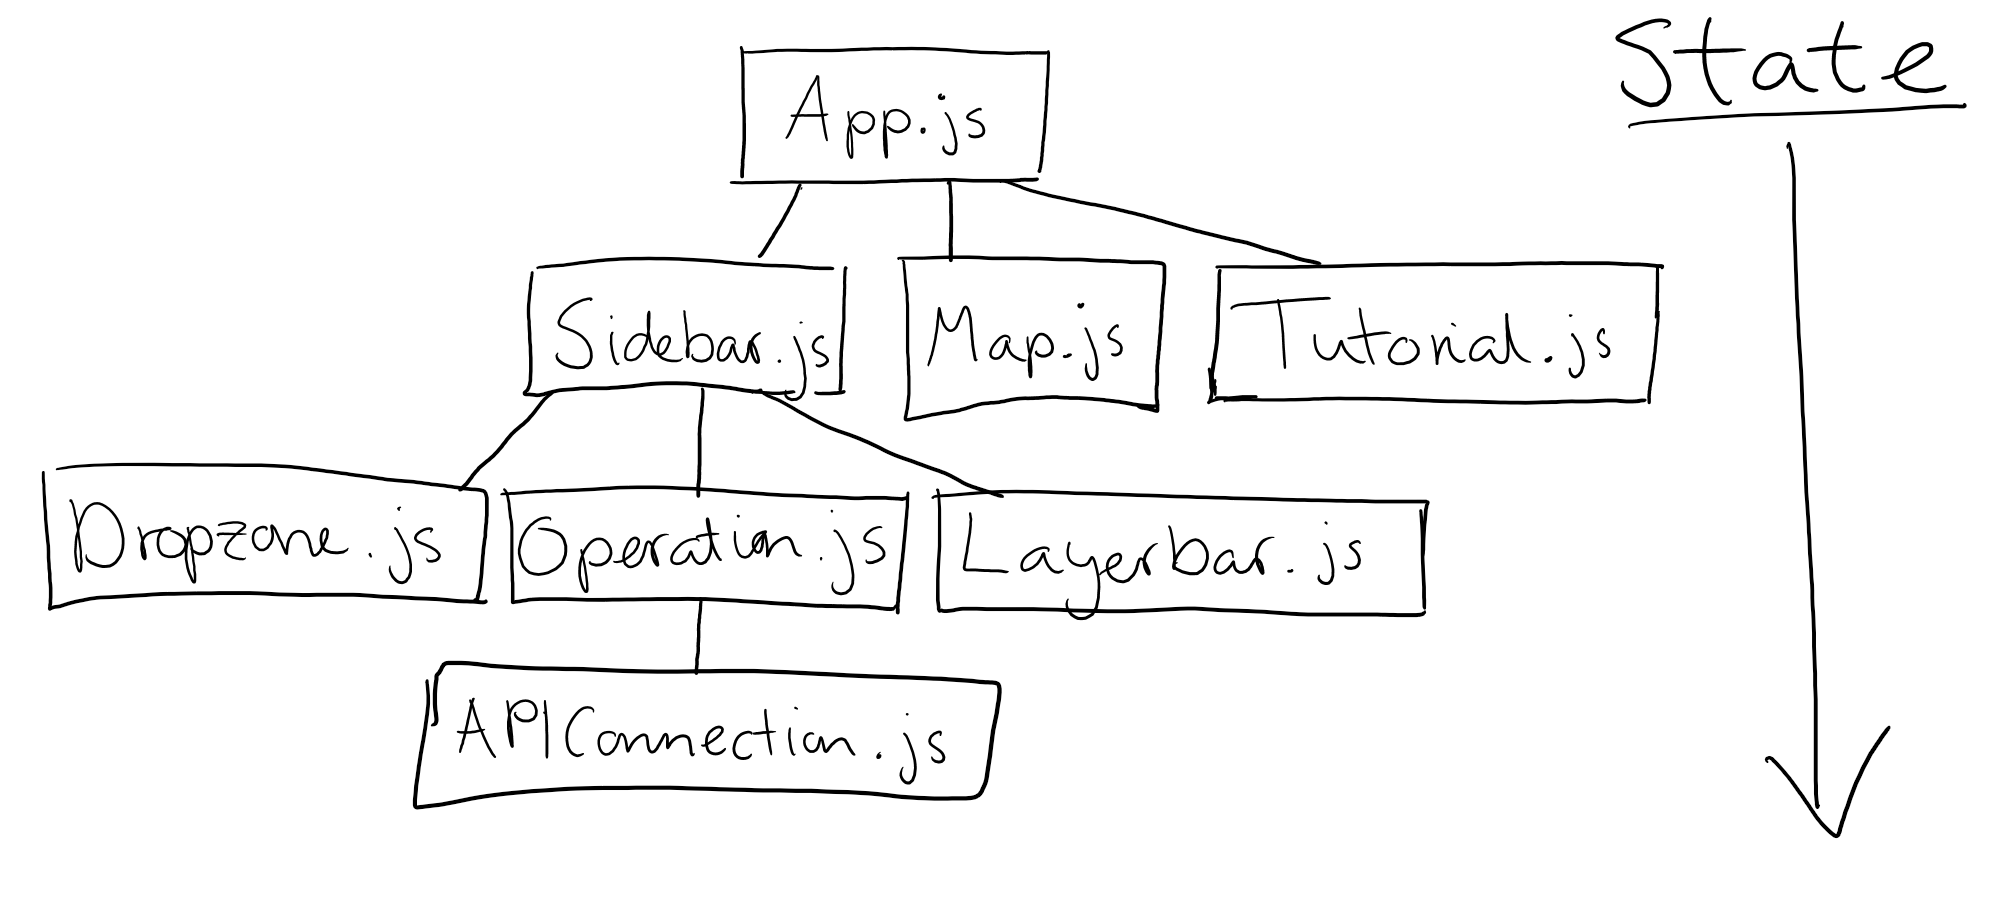
\includegraphics[scale=0.5]{react-arkitektur.PNG}
    \caption{Komponent-diagrammet som viser arv i React-Klienten.}
    \label{fig:react-arkitektur}
\end{figure}

Startpunktet til Serveren er gis\_api.py som importerer app-modulen i prosjektstrukturen. Vanligvis består FLASK-applikasjoner av flere moduler enn api, men i vårt tilfelle importerer app-modulen utelukkende api-modulen. Inne i api-modulen finnes det tre filer som har hovedansvaret for funksjonalitet. Arkitekturen kan sees i figur \ref{fig:api-arktitektur}.

routes.py definerer alle HTTP-endepunktene som serveren skal lytte på og svare på. Hvert endepunkt defineres som en funksjon med såkalte \textit{decorators}, som spesifiserer hvilken URL og HTTP-forespørselstype (GET, PUT, POST, DELETE) som skal matche for å kjøres. Et eksempel er ping-pong-funksjonaliteten nevnt tidligere i prosjektet, se figur \ref{fig:ping-pong}. Alle geoproseseringsoperasjonene har hvert sitt endepunkt, som 'api/buffer' eller 'api/dissolve'.

\begin{figure}[h]
    \center
    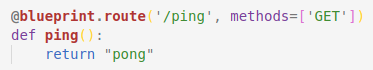
\includegraphics[scale=0.7]{ping-pong-code.png}
    \caption{Eksempel på definisjon av HTTP-endepunkt}
    \label{fig:ping-pong}
\end{figure}



\begin{figure}[h]
    \center
    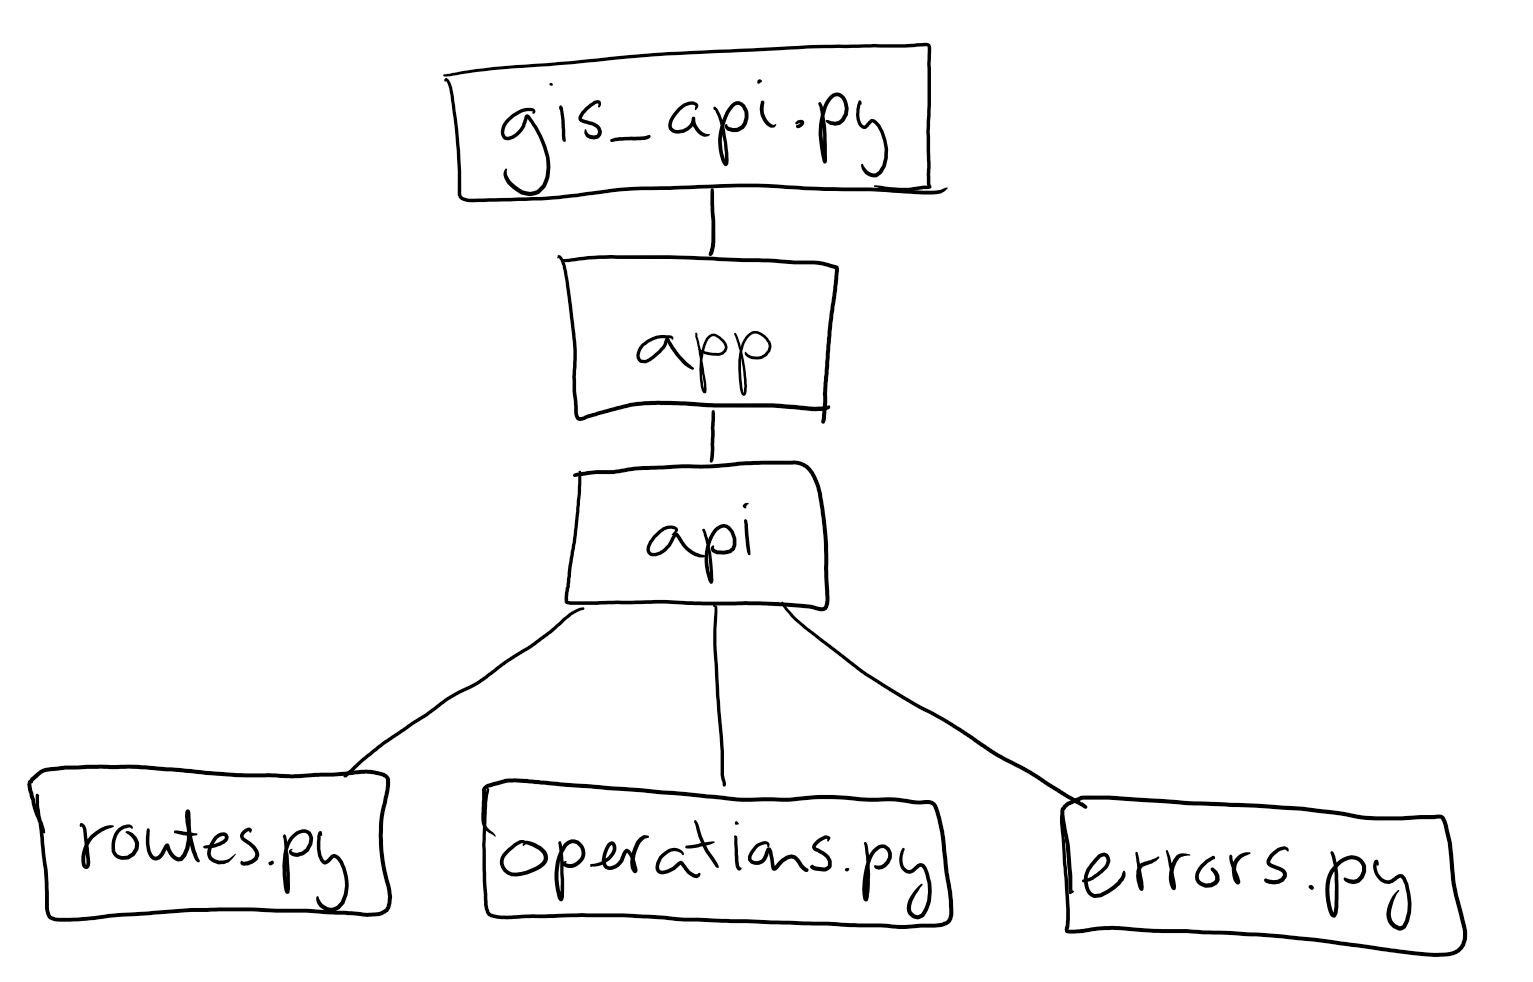
\includegraphics[scale=0.5]{api-arkitektur.PNG}
    \caption{Komponent-diagrammet som viser arv i Python-API'et.}
    \label{fig:api-arktitektur}
\end{figure}

Klienten sender kartdata som en POST-forespørsel til de ulike endepunktene definert i serveren. Endepunktene sender data videre til operations.py, der hver geoprosseringsfunksjon er implementert ved bruk av geopandas. Resultatet sendes tilbake som en respons på HTTP-forespørselen. I tilfelle en feil skjer under utførelsen av HTTP-forespørselen sendes det til errors.py som har ansvaret for å sende tilbake en skreddersydd respons basert på hva som gikk galt. Skreddersydde responser var dessverre ikke mulig å implementere fullstendig. 

Figur \ref{fig:forespørsel} viser flyten når man skal beregne buffer på et kartlag. Klienten gjør klar et HTTP-POST-kall til serveren med riktig endepunkt, buffer-verdi og kartlag. Serveren tar imot forespørselen og beregner bufferen, før den returnerer resultatet til klienten. Det siste klienten gjør er å legge til det nye laget i State og visualisere det i kartet. Denne flyten er representabel for resten av operasjonene i applikasjonen.  

\begin{figure}[h]
    \center
    \includegraphics[scale=0.5]{eksempel-forespørsel.PNG}
    \caption{Flyten mellom Klient og Server for å beregne 100m buffer på en sirkel}
    \label{fig:forespørsel}
\end{figure}

\section{Brukergrensesnitt og brukervennlighet}

Brukergrensesnitt og brukervennlighet går ofte hånd i hånd, ettersom et intuitivt brukergrensesnitt øker brukervennligheten. Gjøremålene i introduksjonen har vært drivende for utformingen av grensesnittet, og i denne underseksjonen skal vi ta for oss de ulike elementene. 

I hovedsak er det kun tre elementer på nettsiden, nemlig sidemeny, kart og tutorial. Alle disse elementene er stylet utifra samme css-stylesheet for å ha samme utforming, se figur \ref{fig:elementer}. Det gjelder fargebruk, skriftstørrelse/skrifttype, avrundede kanter, samme type symboler (hentet fra Material UI). Både sidemenyen og tutorialen har samme skyggelegging og samme avstand over kartet. Dette er hensyn som bevisst er tatt for å skape en helhetsfølelse i applikasjonen. Dette gjør at brukeren enklere kan bruke intuisjon for å ta i bruk de ulike elementene i kartet, ettersom de ser og oppfører seg ganske likt, så har de også en ganske lik måte å fungere på.

\begin{figure}[h]
	\centering
	\begin{subfigure}{.33\textwidth}
		\centering
		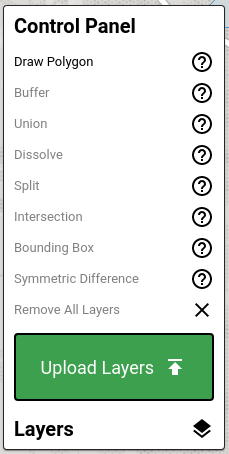
\includegraphics[scale=0.4]{kontrollpanel.png}
		\caption{Kontrollpanel/Sidemeny}
		\label{fig:sub1}
	\end{subfigure}%
	\begin{subfigure}{.33\textwidth}
		\centering
		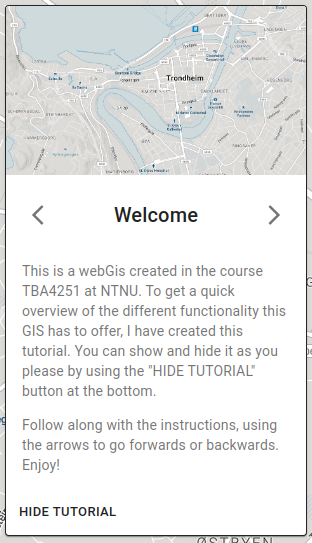
\includegraphics[scale=0.4]{tutorial.png}
		\caption{Tutorial/Brukerveiledning}
		\label{fig:sub2}
    \end{subfigure}
    \begin{subfigure}{.33\textwidth}
		\centering
		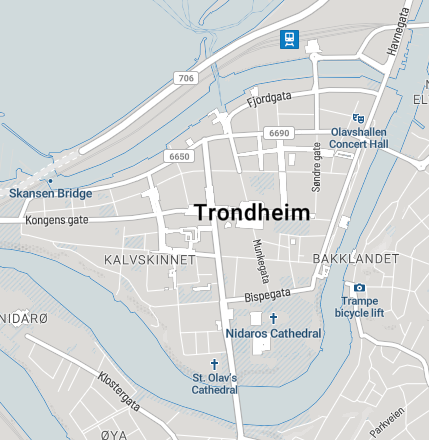
\includegraphics[scale=0.4]{kart.png}
		\caption{Mapbox kart}
		\label{fig:sub2}
	\end{subfigure}
	\caption{\small{De tre hovedelementene som utgjør Klient-applikasjonen.}}
	\label{fig:elementer}
\end{figure}

Brukergrensesnittet består kun av de tre elementene i figur \ref{fig:elementer}, der tutorialen også kan minimeres slik at det kun er to elementer. Det ble gjort et bevisst valg om å holde antall menyer og bokser som var på skjermen nede fordi dette tok oppmerksomheten fra selve kartet. Dette er også et av de egendefinerte gjøremålene, å maksimere kartinteraksjonen, og minimere sidemenybruken. Derfor er det også sånn at det ikke kommer noen store modaler eller pop-up-bokser når man skal bruke de ulike operasjonene. Dette designvalget ga noen utfordringer, ettersom det må være muligheter for både å velge hvilke kartlag man vil ha som input til operasjoner (se seksjon \ref{sec:lagbehandling}), og andre input som foreksempel buffer-størrelse (se seksjon \ref{sec:geoprosessering}). Resultatet har blitt et ryddig, enkelt og forståelig grensesnitt som fortsatt klarer å gi brukeren full kontroll, uten å ta i bruk store og forstyrrende pop-up-bokser, drop-down-menyer og unødig klikking som føles tungvindt og gammeldags ut.

En viktig del av et godt brukergrensesnitt er feedback på handlinger, for å få en forståelse om det man prøvde å gjøre fungerte eller ikke. Alt som kan klikkes eller dras på i applikasjonen har en visuell indikasjon på at man kan gjøre det, enten ved at musepekeren forandrer seg, eller at elementet man holder over endrer farge. I tillegg dukker det opp notifikasjoner nede i venstre hjørne som indikerer om større operasjoner fungerte eller ikke, se figur \ref{fig:success}. Disse meldingene kommer når man har utført HTTP-kall(operasjoner) til Flask-Serveren, eller gjort filopplastinger.  

\begin{figure}[h]
    \center
    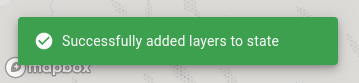
\includegraphics[scale=0.5]{success.PNG}
    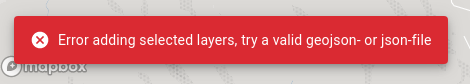
\includegraphics[scale=0.5]{error.PNG}
    \caption{Notifikasjon som indikerer at operasjonen var vellykket eller ikke}
    \label{fig:success}
\end{figure}

For å gjøre kartdesignet i tråd med sidemenyen og tutorialen ble Mapbox Studio tatt i bruk. Mapbox Studio er et nettleser-verktøy laget av Mapbox der man kan endre på grunnkartet som brukes i kart-komponenten. Her kan også brukere laste opp sine egne designs, ta ibruk og endre andre designs. Kartet som er brukt i denne applikasjonen har tatt utgangspunkt i kartet Le Shine av Nathaniel Slaughter \cite{Slaughter}, med noen personlige modifikasjoner til bygningssynlighet på ulike zoom-nivåer for å få det mer i tråd med Mapbox sitt standardkart. Se figur \ref{fig:mapbox-studio}.

\begin{figure}[h]
    \center
    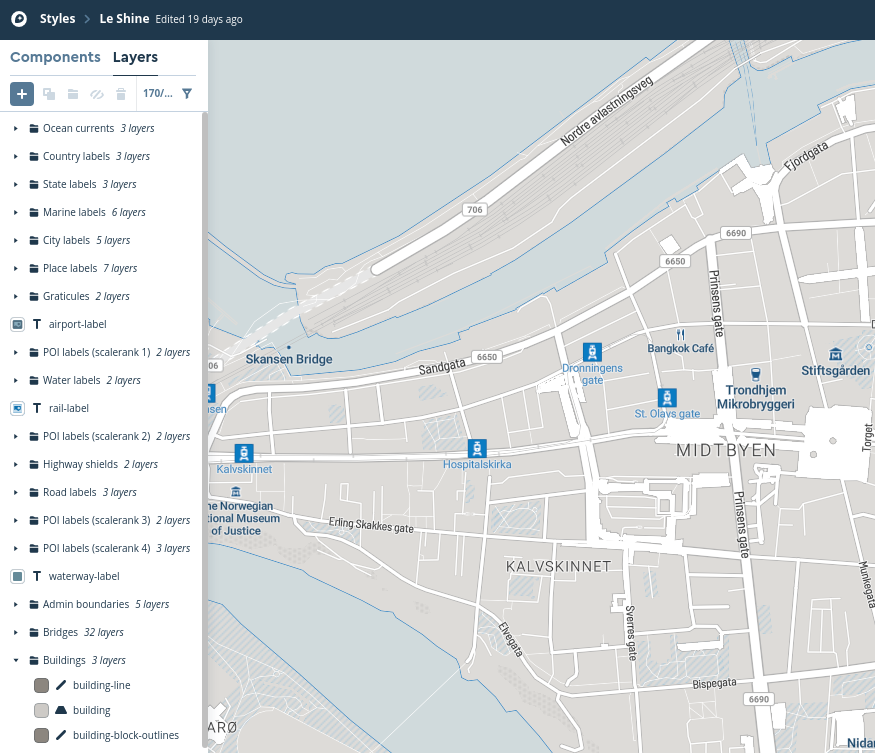
\includegraphics[scale=0.3]{mapbox-studio.png}
    \caption{Screen-capture av mapbox studio med Le Shine-kartet. I sidemenyen kan man se alle kartlagene som utgjør dette custom-kartet}
    \label{fig:mapbox-studio}
\end{figure}

Det siste elementet som skal snakkes om i denne seksjonen er tooltipene til hver operasjon i sidemenyen/kontrollpanelet. I tillegg til brukerveiledningen skal disse tooltipene suplementere brukervennlighet med en enkel forklaring på hva operasjonen gjør og hvor mange lag den trenger for å kunne velges. Ved å ha en lett tilgjengelig tooltip slipper brukeren å bla gjennom brukerveiledningen på nytt hvis hen blir usikker på hva operasjonen faktisk gjore. Informasjonen dukker opp hvis man trykker på spørsmålstegnet knyttet til hver operasjon, som vist i figur \ref{fig:tooltip}. 

\begin{figure}[h]
    \center
    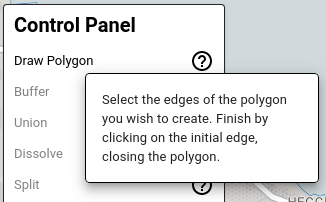
\includegraphics[scale=0.5]{tooltip-polygon.png}
    \caption{Ved å klikke på spørsmålstegnene får man en kjapp presentasjon av hva operasjonen gjør, uten å gå gjennom tutorialen på nytt}
    \label{fig:tooltip}
\end{figure}

\section{Lagbehandling}
\label{sec:lagbehandling}
Denne seksjonen tar for seg de ulike måtene kartlagene kan manipuleres på. Av lagbehandlingsfunksjonene som ble kartlagt i starten av arbeidet ble det valgt å implementere seleksjon, forandring av navn/synlighet, samt opplasting og fjerning av lag. 

\subsubsection{Legge til lag}

Det som ligger i bunn for å legge til lag er å oppdatere App-staten med ny kartdata. Det skjer i funksjonen addLayersToState, denne funksjonen er definert i App, og sendes til alle komponentene som trenger å legge til ny kartdata i applikasjonen. For hver nye geojson-data lages det en unik id og navn til hvert lag, samt en tilfeldig farge som skal brukes i stylingen av laget. Her er det også en sjekk på om det faktisk er minst en feature i laget som legges til, ettersom noen operasjoner kan produsere tomme features. 

\begin{figure}[h]
    \center
    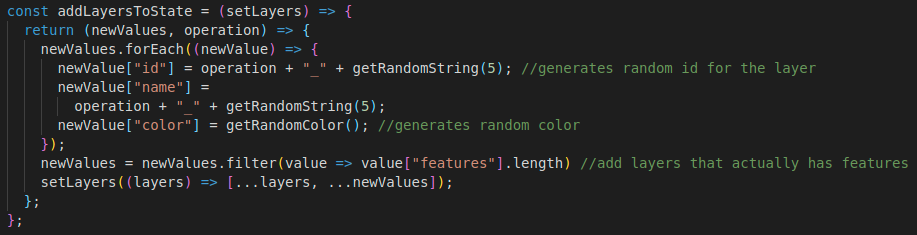
\includegraphics[scale=0.5]{addlayers.png}
    \caption{Funksjonen som legger til nye lag i State}
    \label{fig:addLayers}
\end{figure}

Det er to måter å legge til nye, egne lag i applikasjonen. Den første metoden, filopplasting, er implementert ved bruk av React-biblioteket Dropzone. Dette er en komponent som kan ta imot filer, enten ved at man drar dem inn i komponenten, eller klikker på den for å få opp en filutforsker. Etter at en fil er godtatt av komponenten sendes innholdet til en 'useCallback'-funksjon(se figur \ref{fig:usecallback}) hvor man må definere hva som skal skje videre. Siden FileReader-funksjonen er asynkron må man først lage en liste av av promises, der hvert promise er avlesningen av hvert lag som er lagt til. Når alle filene har blitt lest inn blir Promise.all() trigget, som legger til filene i staten ved bruk av funksjon \ref{fig:addLayers}.

\begin{figure}[h]
    \center
    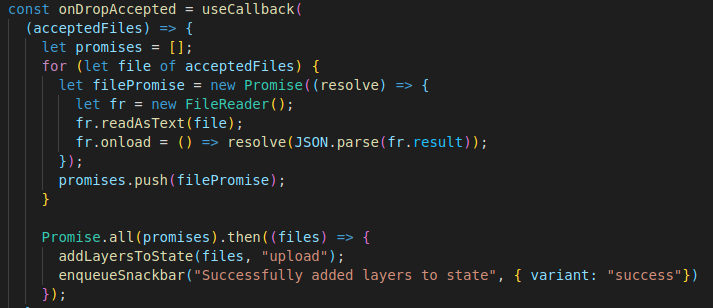
\includegraphics[scale=0.5]{usecallback.png}
    \caption{useCallBack-funksjonen som kjøres når filene i dropzone har blitt godkjent.}
    \label{fig:usecallback}
\end{figure}

Den andre metoden for å lage helt nye lag er en av operasjonene i sidemenyen, nemlig 'Draw Polygon'. Draw-funksjonaliteten er en tilleggsmodul til Mapbox GL, som eksplisitt er implementert i denne applikasjonen. Draw-funksjonen er instansiert i App, og sendt videre til både kart-komponenten og sidebaren. Etter man har streket opp et polygon med tegneverktøyet til Draw (Som aktiveres når man trykker på draw polygon), sendes dataen til en lignende useCallBack, som igjen legger laget til ved bruk av funksjon \ref{fig:addLayers}.

\subsubsection{Fjerne lag}

Det å fjerne lag kan gjøres to steder, enten ved å trykke på remove all layers i sidemenyen, eller å fjerne individuelle lag ved å trykke på søppelkasse-ikonet i layers-oversikten (se figur \ref{fig:layerbar}).  

\begin{figure}[h]
    \center
    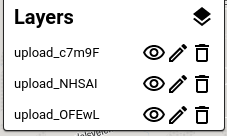
\includegraphics[scale=0.5]{layers.png}
    \caption{Layerbar-komponenten som er en del av sidemenyen}
    \label{fig:layerbar}
\end{figure}

\subsubsection{Seleksjon av kartlag}

\subsubsection{Forandre navn og synlighet}

\section{Geoprosessering}
\label{sec:geoprosessering}
\subsubsection{Buffer}
\subsubsection{Union}
\subsubsection{Dissolve}
\subsubsection{Split}
\subsubsection{Intersection}
\subsubsection{Bounding Box}
\subsubsection{Symmetric Difference}

\section{Tutorial}

- Komponent

-- Bilde

-- Piler

-- Tekst

\section{Dokumentasjon}

For å 

- Doc-strings

\section{Hosting}
\label{sec:hosting}
Som tidligere nevnt er Klient-delen av applikasjonen hostet via github pages. Github pages er en tjeneste knyttet til kildekode publisert på github, som bygger og deployer prosjekter, samt tilgjengeligjører dem på internett. Vanligvis er nettadressen til prosjektene knyttet til github-brukeren til den som eier prosjektet (i mitt tilfelle torsol.github.io/<prosjektnavn>), men ikke her, fordi jeg bruker et eget domene. React har et eget bibliotek som integerer prosjekter med github pages, så det eneste som trengs for å rulle ut en ny versjon av applikasjonen er å kjøre et script i kommandolinjen. 

Server-delen av applikasjonen kan ikke hostes på github pages, dette er fordi github pages kun fungerer for statiske nettsider i html, css og javascript. Derfor tok man i bruk heroku istedenfor. Ved å integrere heroku med github-kontoen ble det laget en pipeline som bygger og deployer en ny versjon av serveren for hver gang master-branchen oppdateres. 

Ved å ta ibruk både github pages og heroku oppnådde man gjøremålet om at programmet ikke forsvinner med studentbruker. I tillegg tilbyr begge løsningene rask prototyping, med lynrask respons fra endring til det er live på nettet. 
